\section{Реализация}

\subsubsection*{Необходимо реализовать:}
\begin{itemize}
    \item Структуру автоматона, функции для работы с ним
    \item Общие операции для решеток (join, meet, strictEquals, ...)
    \item Операции на строках (length, concat, substring, ...)
    \item Оператор замыкания (widening)
\end{itemize}

\subsubsection*{Дополнительные требования:}
\begin{itemize}
    \item Есть тестовый датасет из 23 и 62 реальных проектов
    \item Время исполнения не должно увеличиться более чем на $20\%$
    \item Потребление памяти не должно увеличиться более чем на $10\%$
\end{itemize}

\newpage
\subsection{Структура}
Сама структура автомата базовая - есть вершины (states) и переходы между ними. Некоторые из стейтов помечены как начальные или как конечные. На переходах стоят строки или символ $\top$, обозначающий любую строку

\subsubsection*{union}
Основной операцией является объединение автоматов. С её помощью находим наименьший язык, содержащий оба, порождаемых автоматами

Реализаиця простая: создаем общее начальное состояние, проводим из него переходы с пустой строкой в начальные состояния двух объединяемых автоматов. Затем минимизируем полученный автомат (чуть ниже описана функция minimize)

\subsubsection*{intersect}
Еще одной важной операцией является пересечение автоматов. Она позволяет понять, есть ли в двух алфавитах общие слова. А также находить наибольший общий подъязык

Реализуется она при помощи операций дополнения и объединения, то есть по формуле \[A \cap B = S / ((S / A) \cup (S / B))\]

Дополнение строится таким образом - выписываем все возможные переходы в обоих автоматах, а затем для каждого переходы между двумя вершинами заменяются на дополнение к этим переходам

\subsubsection*{subset}
Проверка на то, что один язык полностью содержит другой. Реализуется с помощью дополнения и пересечения по формуле
\[A \subset B <=> (S / B) \cap A = \emptyset\]

\subsubsection*{minimize}
Убирает лишние вершины и переходы. Например может произойти так, что из одной вершины ведут 2 перехода с одинаковой строкой. Тогда можно упростить автомат так, чтобы склеились 2 вершины в одну. Также избавляемся от переходов по пустой строке

Алгоритм минимизации такой - сначала проверяем, является ли автомат детерменированным, то есть что нет двух исходящих переходов из одной вершины с одинаковыми символами на них. А также что нет пустых переходов. Если есть, то склеиваем эти 2 вершины. Это операция детерменирования

Затем, чтобы избавиться от двух одинаковых входящих переходов, мы делаем reverse, то есть перенаправляем все ребра и помечаем конечные вершины начальными и наоборот. Теперь вызываем еще раз determinize. Повторив еще раз reverse + determinize, получим начальный автомат, но без лишних переходов и вершин

Последним шагом удаляем те вершины, из которых нельзя попасть в финальные. Таким образом получим упрощенную версию того же самого автомата

\newpage
\subsection{Операции для решеток}
Операции join и meet аналогичны union и intersect для автоматов. Остается только разобрать случаи, когда один из аргументов $\top$ или $\bot$. 

\subsubsection*{strictEquals}
Проверяем, что 2 автомата порождают одинаковые языки. В общем случае можем проверить то, что один язык включается в другой и наоборот. Однако операция пересечения слишком громоздкая (нужно сделать 3 раза дополнение), поэтому для конечных языков проще выписать 2 порождаемых языка и проверить их на соответствие. Язык является конечным, если в нем нет $\top$ переходов и циклов

\subsubsection*{equals}
В отличие от strictEquals, equals проверяет то, что есть хоть одно общее слово. Опять это можно сделать при помощи пересечения, но для конечных лучше сравнивать языки

\newpage
\subsection{Операции на строках}
\subsubsection*{Length}
Возвращает интервал $[c_1, c_2]$, такой что $c_1 \leq |s| \leq c_2$. При этом если $s$ содержит в себе цикл, или же содержит в себе переход, на котором стоит $\top$, то есть любая строка, то максимальная длина будет сколь угодно большой. Минимальная при этом заменяет все топы на пустые строки.
\begin{figure}[H]
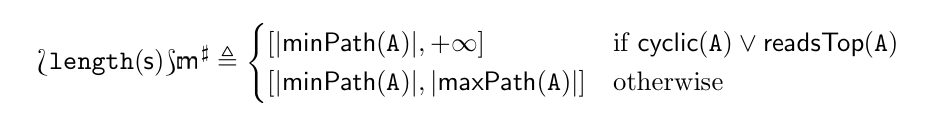
\includegraphics[width=\textwidth]{images/tarsis-length.png}\hfill
\end{figure}
    

\subsubsection*{Concat}
\subsubsection*{Contains}

\begin{figure}[H]
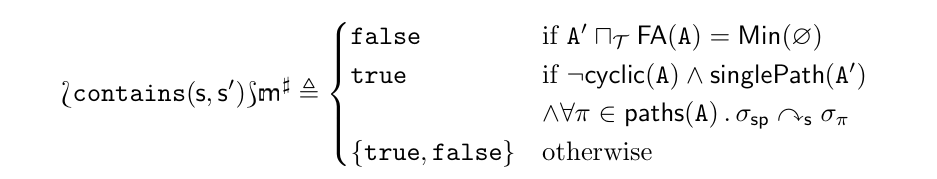
\includegraphics[width=\textwidth]{images/tarsis-contains.png}\hfill
\end{figure}
        
\subsubsection*{IndexOf}

\subsubsection*{Substr}

\subsubsection*{Replace}